%===============================================================================
% LaTeX sjabloon voor de bachelorproef toegepaste informatica aan HOGENT
% Meer info op https://github.com/HoGentTIN/bachproef-latex-sjabloon
%===============================================================================

\documentclass{bachproef-tin}

\usepackage{hogent-thesis-titlepage} % Titelpagina conform aan HOGENT huisstijl\\

%%---------- Documenteigenschappen ---------------------------------------------

% De titel van het rapport/bachelorproef
\title{Benchmarken van geïntegreerde ontwikkelingsomgevingen om de geschikte ontwikkelingsomgevingen te bepalen}

% Je eigen naam
\author{Lorin Speybrouck}

% De naam van je promotor (lector van de opleiding)
\promotor{Jan Willem}

% De naam van je co-promotor. Als je promotor ook je opdrachtgever is en je
% dus ook inhoudelijk begeleidt (en enkel dan!), mag je dit leeg laten.
\copromotor{}

% Indien je bachelorproef in opdracht van/in samenwerking met een bedrijf of
% externe organisatie geschreven is, geef je hier de naam. Zoniet laat je dit
% zoals het is.
\instelling{---}

% Academiejaar
\academiejaar{2021-2022}

% Examenperiode
%  - 1e semester = 1e examenperiode => 1
%  - 2e semester = 2e examenperiode => 2
%  - tweede zit  = 3e examenperiode => 3
\examenperiode{2}

%===============================================================================
% Inhoud document
%===============================================================================

\begin{document}

%---------- Taalselectie -------------------------------------------------------
% Als je je bachelorproef in het Engels schrijft, haal dan onderstaande regel
% uit commentaar. Let op: de tekst op de voorkaft blijft in het Nederlands, en
% dat is ook de bedoeling!

%\selectlanguage{english}

%---------- Titelblad ----------------------------------------------------------
\inserttitlepage

%---------- Samenvatting, voorwoord --------------------------------------------
\usechapterimagefalse
%%=============================================================================
%% Voorwoord
%%=============================================================================

\chapter*{\IfLanguageName{dutch}{Woord vooraf}{Preface}}
\label{ch:voorwoord}

%% TODO:
%% Het voorwoord is het enige deel van de bachelorproef waar je vanuit je
%% eigen standpunt (``ik-vorm'') mag schrijven. Je kan hier bv. motiveren
%% waarom jij het onderwerp wil bespreken.
%% Vergeet ook niet te bedanken wie je geholpen/gesteund/... heeft

Deze scriptie is geschreven ter afsluiting van de opleiding Toegepaste Informatica van
de Hogeschool Gent.

Het onderwerp van deze scriptie heb ik bedacht omdat ik al een interesse had in het werken met IDEs en dit op een zo efficiënt mogelijke manier te doen. Op het eerste zicht was er niet veel informatie over dit onderwerp terug te vinden, zeker niet over uitvoeren van de performantie testen, maar ik wou mijn onderzoek toch over dit onderwerp doen. Gaandeweg heb ik wel de nodige informatie gevonden in tech-manuals van de IDEs, forums waar technische problemen besproken werden en boeken die de IDEs beschrijven.

Graag wil ik mijn promotor, Jan Willem, bedanken voor de begeleiding tijdens
deze bachelorproef.
%%=============================================================================
%% Samenvatting
%%=============================================================================

% TODO: De "abstract" of samenvatting is een kernachtige (~ 1 blz. voor een
% thesis) synthese van het document.
%
% Deze aspecten moeten zeker aan bod komen:
% - Context: waarom is dit werk belangrijk?
% - Nood: waarom moest dit onderzocht worden?
% - Taak: wat heb je precies gedaan?
% - Object: wat staat in dit document geschreven?
% - Resultaat: wat was het resultaat?
% - Conclusie: wat is/zijn de belangrijkste conclusie(s)?
% - Perspectief: blijven er nog vragen open die in de toekomst nog kunnen
%    onderzocht worden? Wat is een mogelijk vervolg voor jouw onderzoek?
%
% LET OP! Een samenvatting is GEEN voorwoord!

%%---------- Nederlandse samenvatting -----------------------------------------
%
% TODO: Als je je bachelorproef in het Engels schrijft, moet je eerst een
% Nederlandse samenvatting invoegen. Haal daarvoor onderstaande code uit
% commentaar.
% Wie zijn bachelorproef in het Nederlands schrijft, kan dit negeren, de inhoud
% wordt niet in het document ingevoegd.

\IfLanguageName{english}{%
\selectlanguage{dutch}
\chapter*{Samenvatting}
\lipsum[1-4]
\selectlanguage{english}
}{}

%%---------- Samenvatting -----------------------------------------------------
% De samenvatting in de hoofdtaal van het document

\chapter*{\IfLanguageName{dutch}{Samenvatting}{Abstract}}

Vandaag de dag zijn er verschillende mogelijkheden voor software ontwikkelaars om geholpen te worden bij het schrijven van programmas door Integrated Developper Environements of IDEs, maar welke hiervan zijn het meest performant? Dit word onderzocht omdat hoe minder een ontwikkelaar op zijn IDE moet wachten hoe meer hij productief kan werken.

Er bestaan verschillende soorten IDEs op de markt. Sommige zijn gratis en sommige betalend. Sommige zijn toegelegd op een specifieke taal en anderen zijn algemeen bruikbaar en makkelijk customiseerbaar. Als laatste moet er ook het onderscheid gemaakt worden tussen echte IDEs, die het hele ontwikkelingsproces van een programma ondersteunen, en code editors die minimale functionaliteit hebben. De vraag die dit onderzoek wil beantwoorden is welke IDE het meest performant is op verschillende aspecten. Deze aspecten zijn de opstart tijd, de zoektijd in bestanden, de build tijd van code en het CPU en RAM gebruik in de idle stand. 
Ter beantwoording van de probleemstelling zijn volgende deelvragen geformuleerd

\begin{itemize}
    \item Welke IDE is het meest performant op de aspecten van opstart tijd, zoektijd in bestanden, build tijd van code en CPU en RAM gebruik?
    \item Heeft de keuze van project en de programmeertaal waar die in geschreven is een effect op de opstart tijd, zoektijd in bestanden, build tijd van code en CPU en RAM gebruik?
\end{itemize}

Het onderzoek werd uitgevoerd met 2 testprojecten: Cake en Mindustry, daarnaast werden er 5 IDEs onderzocht: VS Code, Visual Studio, Eclipse, Notepad++ en IntelliJ.

De verwachtingen waren dat VS Code het beste zou scoren op performantie aangezien dit de meest populaire en gebruikte IDE is. Dit werd ook bevestigd in dit onderzoek. Ook zijn Visual Studio en IntelliJ goede opties die meer functionaliteit aanbieden en een grotere performantie impact hebben.

Er werd ook opgemerkt dat de prestaties van de IDE grotendeels onafhankelijk zijn van de taal waarin het project geschreven.

Tot slot is er in dit onderzoek opgemerkt dat er bij het builden van C\# code een groot verschil in uitvoertijd, tot 2 maal zo lang, zit tussen de uitvoerende IDEs. Hier is meer onderzoek voor nodig aangezien deze dezelfde onderliggende commando's gebruiken.

De details van het onderzoek zijn te vinden in het volgende deel van deze scriptie.


%---------- Inhoudstafel -------------------------------------------------------
\pagestyle{empty} % Geen hoofding
\tableofcontents  % Voeg de inhoudstafel toe
\cleardoublepage  % Zorg dat volgende hoofstuk op een oneven pagina begint
\pagestyle{fancy} % Zet hoofding opnieuw aan

%---------- Lijst figuren, afkortingen, ... ------------------------------------

% Indien gewenst kan je hier een lijst van figuren/tabellen opgeven. Geef in
% dat geval je figuren/tabellen altijd een korte beschrijving:
%
%  \caption[korte beschrijving]{uitgebreide beschrijving}
%
% De korte beschrijving wordt gebruikt voor deze lijst, de uitgebreide staat bij
% de figuur of tabel zelf.

\listoffigures
\listoftables

% Als je een lijst van afkortingen of termen wil toevoegen, dan hoort die
% hier thuis. Gebruik bijvoorbeeld de ``glossaries'' package.
% https://www.overleaf.com/learn/latex/Glossaries

%---------- Kern ---------------------------------------------------------------

% De eerste hoofdstukken van een bachelorproef zijn meestal een inleiding op
% het onderwerp, literatuurstudie en verantwoording methodologie.
% Aarzel niet om een meer beschrijvende titel aan deze hoofstukken te geven of
% om bijvoorbeeld de inleiding en/of stand van zaken over meerdere hoofdstukken
% te verspreiden!

%%=============================================================================
%% Inleiding
%%=============================================================================

% De inleiding moet de lezer net genoeg informatie verschaffen om het onderwerp te begrijpen en in te zien waarom de onderzoeksvraag de moeite waard is om te onderzoeken. In de inleiding ga je literatuurverwijzingen beperken, zodat de tekst vlot leesbaar blijft. Je kan de inleiding verder onderverdelen in secties als dit de tekst verduidelijkt. Zaken die aan bod kunnen komen in de inleiding~\autocite{Pollefliet2011}:

%\begin{itemize}
%    \item context, achtergrond
%    \item afbakenen van het onderwerp
%    \item verantwoording van het onderwerp, methodologie
%    \item probleemstelling
%    \item onderzoeksdoelstelling
%    \item onderzoeksvraag
%    \item \ldots
%\end{itemize}

\chapter{\IfLanguageName{dutch}{Inleiding}{Introduction}}
\label{ch:inleiding}

De job van een programmeur is complex met verschillende verantwoordelijkheden. Dit gaat van het effectieve schrijven van nieuwe code tot het testen van deze code, het opsporen van fouten, het beheren van verschillende versies... Om deze lasten te verminderen zijn er over de jaren heen verschillende geïntegreerde ontwikkelingsomgeving (IDEs) op de markt gekomen, met het doel de productiviteit van de programmeur te verhogen. 

IDEs zijn ver gekomen sinds het idee ten eerste werd voorgesteld in de 1980 \autocite{Kline2005}. De eerste versies waren onhandig in gebruik en vereisten meerdere uren professionele training om effectief gebruikt te kunnen worden. Deze programma’s hadden wel het potentieel om programmeurs productiever te laten worden, maar door de grote leercurve verkozen vele de gewone tekst-editor. De kost van de eerste software was ook een grote barrière, deze kon makkelijk oplopen tot \$20,000 per ontwikkelaar. Hedendaags gebruikt bijna iedere programmeur een IDE en deze zijn vaak gratis en open source.

Maar er is geen overzicht van de performantie van moderne IDEs, om een geïnformeerde keuze te kunnen maken en niet enkel naar populariteit te kijken. Dit tracht dit onderzoek te doen, om van enkele van de meest populaire IDEs, zoals gevonden in de \autocite{StackOverflow2021} Developer Survey, de performantie te testen. De IDEs opgenomen in dit onderzoek zijn Visual Studio Code, Visual Studio, Eclipse, IntelliJ, en Notepad++.

\newpage

\section{Onderzoeksvraag}

Dit onderzoek heeft als doel de volgende onderoeksvragen te beatwoorden

\begin{itemize}
    \item Welke IDE is het meest performant op de aspecten van opstart tijd, zoektijd in bestanden, build tijd van code en CPU en RAM gebruik?
    \item Heeft de keuze van project en de programmeertaal waar die in geschreven is een effect op de opstart tijd, zoektijd in bestanden, build tijd van code en CPU en RAM gebruik?
\end{itemize}

\section{Onderzoeksdoelstelling}

In de vorm van een vergelijkend onderzoek worden eerst de voorgenoemde performantie aspecten getest met verschillende scripts en daarna vergeleken. Dit om uiteindelijk te kunnen bepalen wat de meest performante IDE op de markt is op algemene vlakken, maar ook extra toegelegd op Java en C\# programmatie.

\section{\IfLanguageName{dutch}{Opzet van deze bachelorproef}{Structure of this bachelor thesis}}
\label{sec:opzet-bachelorproef}

% Het is gebruikelijk aan het einde van de inleiding een overzicht te
% geven van de opbouw van de rest van de tekst. Deze sectie bevat al een aanzet
% die je kan aanvullen/aanpassen in functie van je eigen tekst.

De rest van deze bachelorproef is als volgt opgebouwd:

In Hoofdstuk~\ref{ch:stand-van-zaken} wordt een overzicht gegeven van de stand van zaken binnen het onderzoeksdomein, op basis van een literatuurstudie.

In Hoofdstuk~\ref{ch:methodologie} wordt de methodologie toegelicht en worden de gebruikte onderzoekstechnieken besproken om een antwoord te kunnen formuleren op de onderzoeksvragen.

Tenslotte wordt een antwoord geformuleerd op de onderzoeksvragen en een conclusie
toegelicht op het onderzoek in Hoofdstuk~\ref{ch:conclusie}. Daarbij wordt er ook een aanzet gegeven voor toekomstig onderzoek als gevolg van een onverklaarde vinding in deze studie.

\chapter{\IfLanguageName{dutch}{Stand van zaken}{State of the art}}
\label{ch:stand-van-zaken}

% Tip: Begin elk hoofdstuk met een paragraaf inleiding die beschrijft hoe
% dit hoofdstuk past binnen het geheel van de bachelorproef. Geef in het
% bijzonder aan wat de link is met het vorige en volgende hoofdstuk.

% Pas na deze inleidende paragraaf komt de eerste sectiehoofding.

De literatuurstudie geeft een beeld van welke programma’s in dit onderzoek worden opgenomen. Voordat deze IDEs worden besproken, wordt er eerst een definitie opgesteld van de IDE en de source code editor, om het verschil duidelijk te maken. Daarna volgt er een geschiedenis van het opkomen van de IDE alsook de nood van de moderne IDE in de ontwikkelingsomgeving. Als laatste worden de aanbevolen systeemvereisten aangehaald zodat er al een beeld gevormd kan worden van hoe de verschillende IDEs zullen presteren.

\section{\IfLanguageName{dutch}{IDE en Source Code Editor}{IDE and Source Code Editor}}
\label{sec:IDE-codeEditor}

De termen IDE en source code editor, meestal verkort tot code editor, worden vaak door elkaar gebruikt. Er is daarentegen een functioneel verschil tussen deze twee termen. Het verschil wordt verduidelijkt met de volgende definitie:

\begin{displayquote}
"An integrated development environment (IDE) is software for building applications that combines common developer tools into a single graphical user interface (GUI). An IDE typically consists of a Source code editor,  Local build automation and Debugger." \autocite{RedHat2018}
\end{displayquote}

De code editor maakt dus integraal deel uit van de IDE. Deze laatste bevat daarnaast namelijk andere tools zoals een geïntegreerde compiler/interpreter, build-automatisatie, een debugger, versiecontrole, een test framework en soms nog andere tools. Voorbeelden van IDEs in dit onderzoek zijn Visual Studio, Eclipse en IntelliJ.

Onder code editor wordt verstaan dat dit een grafische tekst editor is met extra functionaliteit zoals syntax markering, indentatie, auto-voltooiing en bracket matching. Hieruit kan ook afgeleid worden dat code editors lagere hardware vereisten hebben doordat deze minder functionaliteit hebben. Moderne code editors maken vaak gebruik van plug-ins of extensions om meer functionaliteiten van de IDE aan te bieden. Maar in het algemeen bieden ze dit niet standaard aan en moet de gebruiker dit zelf configureren.

\begin{figure}[h!]
    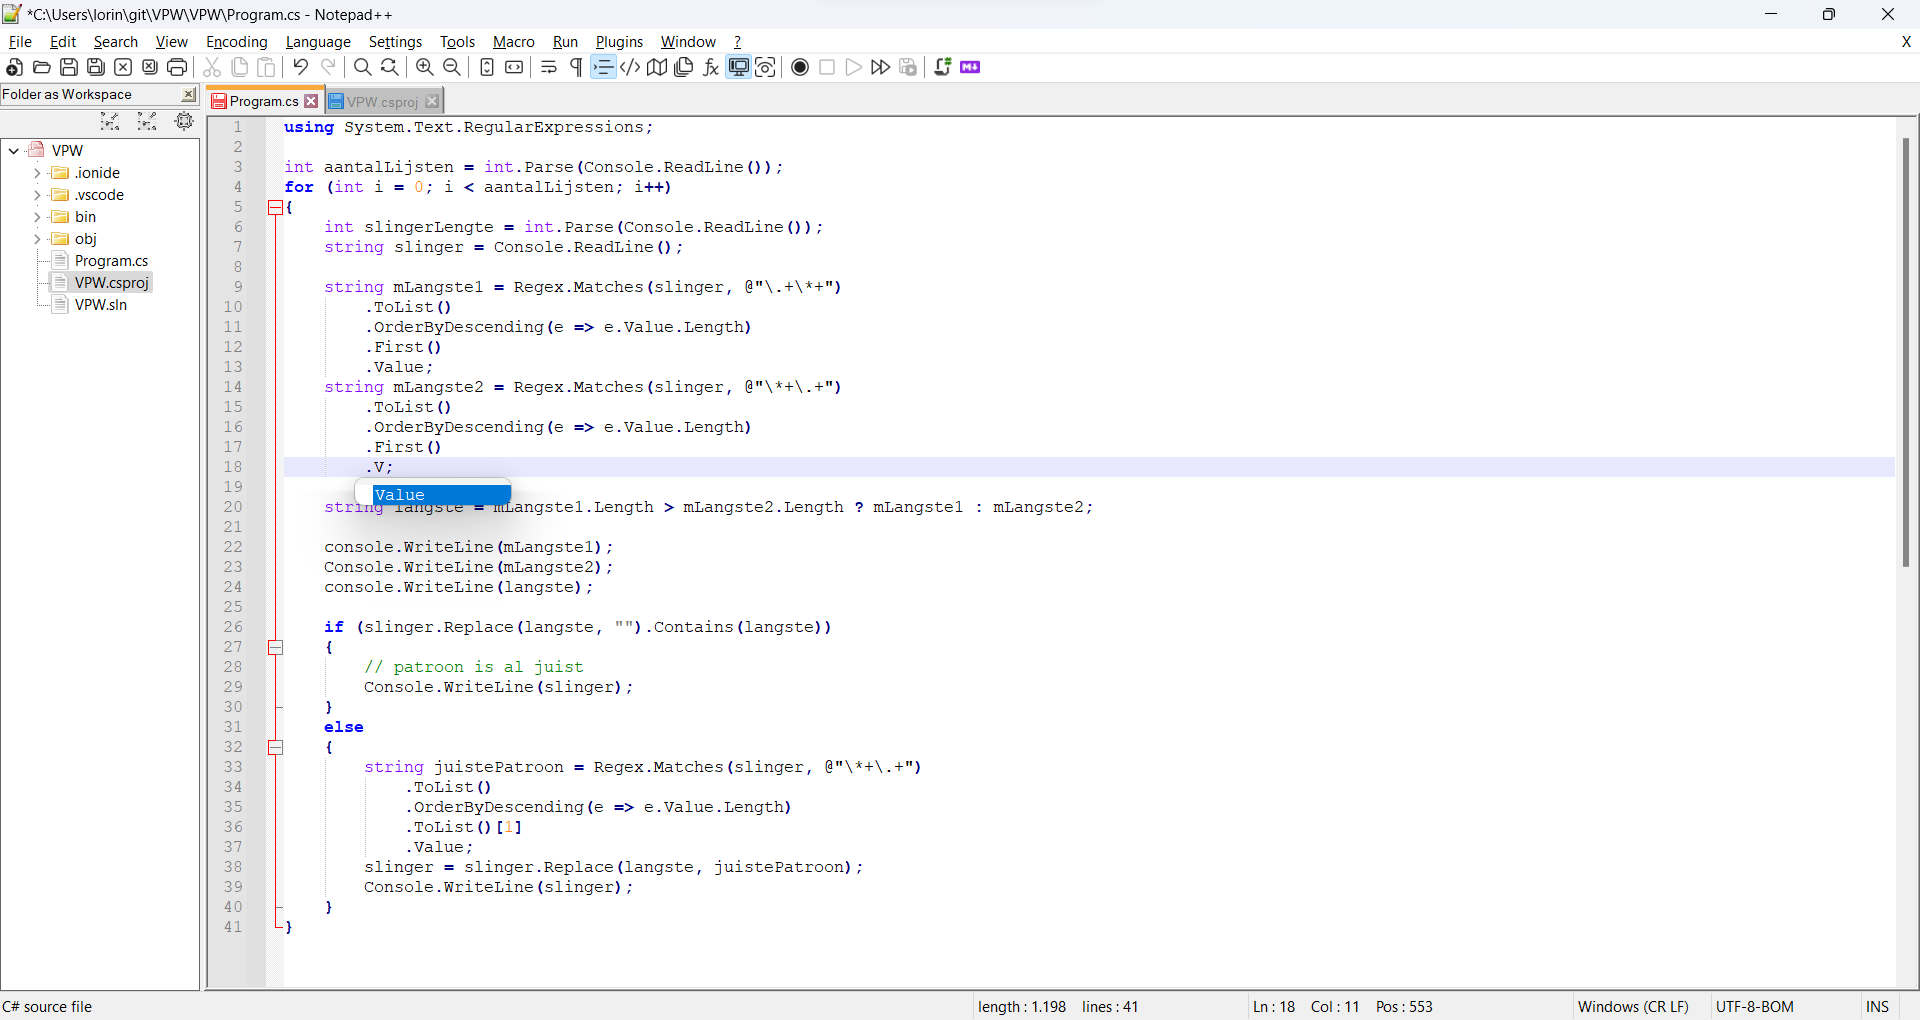
\includegraphics[width=\linewidth]{CodeEditor.png}
    \caption{De Notepad++ code editor}
    \label{fig:codeEditor}
\end{figure}

\begin{figure}[h!]
    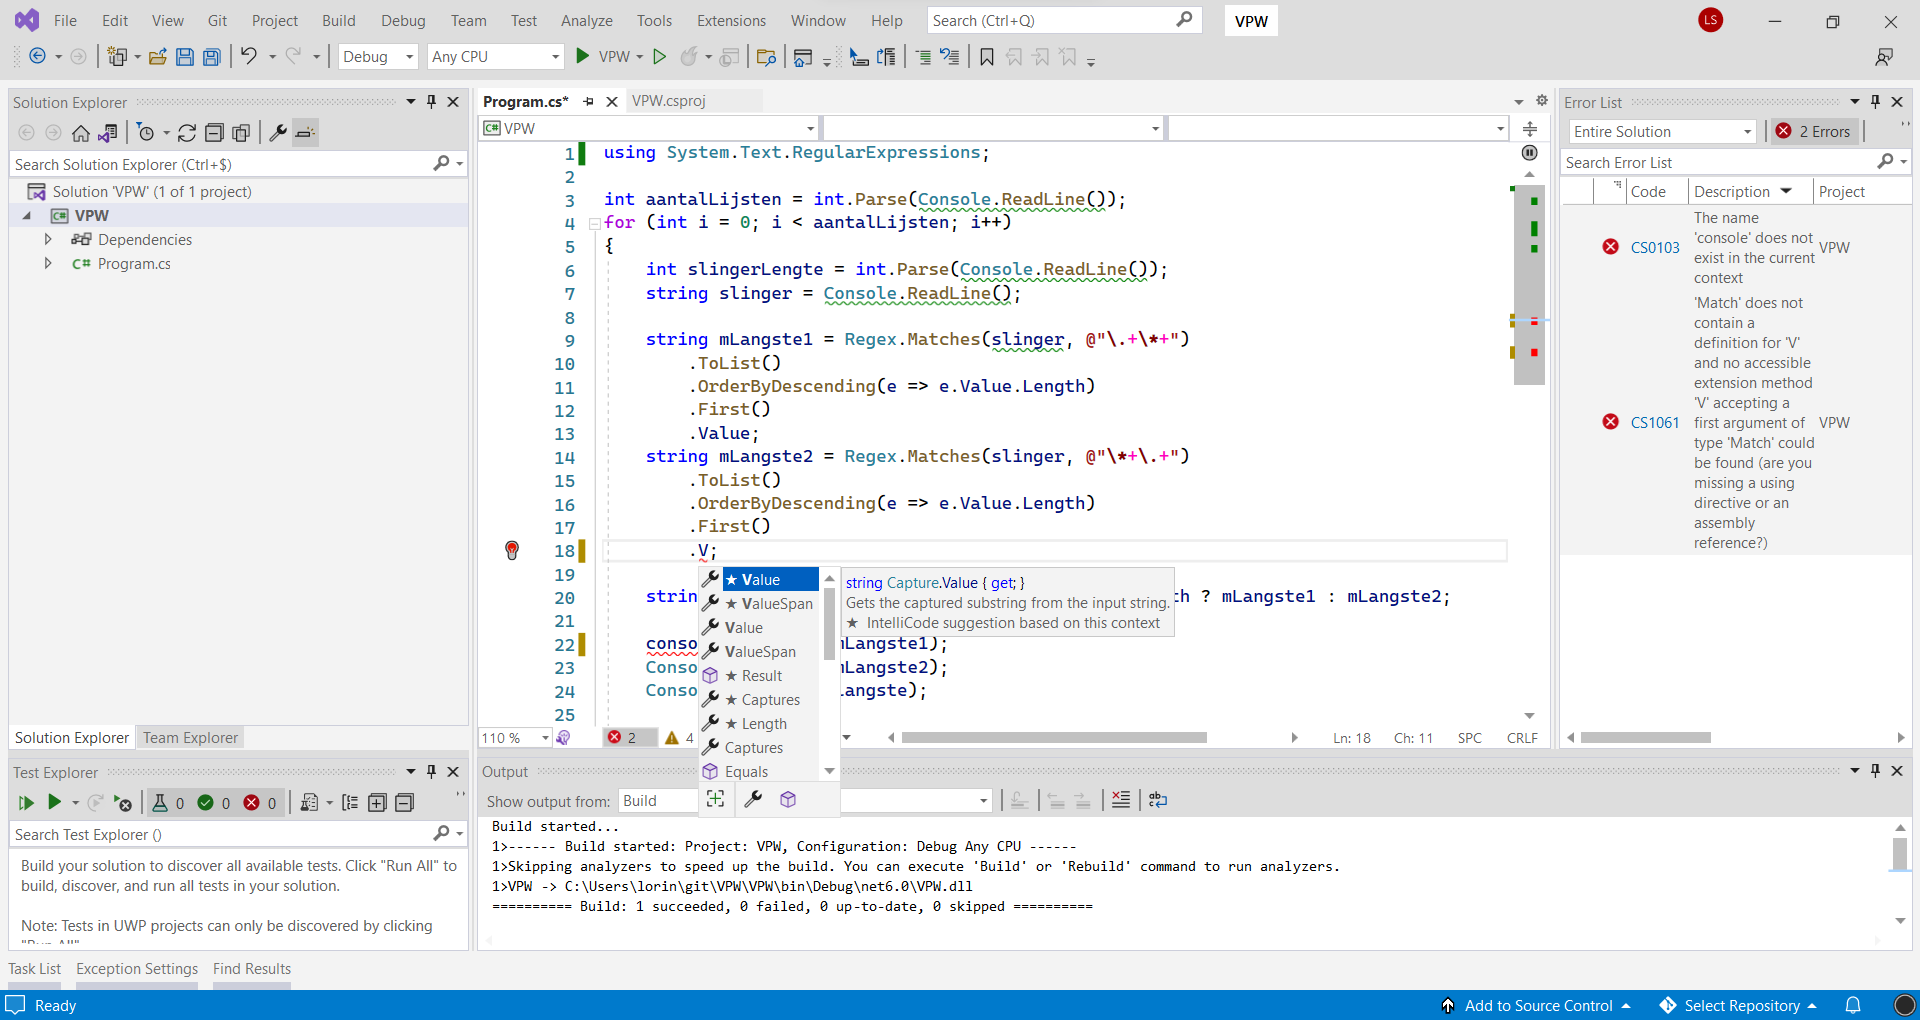
\includegraphics[width=\linewidth]{IDE.png}
    \caption{De Visual Studio IDE}
    \label{fig:IDE}
\end{figure}

Als illustratie zijn 2 afbeeldingen van hetzelfde project gegeven om het verschil in functionaliteit tussen de code editor en de IDE te verduidelijken. Op het eerste gezicht zijn deze vrij gelijkend, een tekst editor die centraal staat met daarrond wat vensters en knoppen. Maar bij nader inzicht is het duidelijk dat de IDE meer aanbiedt, zoals sterkere syntax markering(meer sleutelwoorden worden gekleurd), context bewuste aanvulling (het menu onderaan de V), error controle(lijst van errors en rood onderlijnde code), build en run uitvoer, testen, debugging via breakpoints...

\section{\IfLanguageName{dutch}{Ontstaan van de IDE}{Origin of the IDE}}
\label{sec:IDE-ontstaan}

De eerste IDE is ontwikkeld in 1980, nadat programmeertalen overschakelden naar ontwikkeling via de console. Dit was hiervoor niet mogelijk omdat de eerste software geprogrammeerd werd met ponskaarten. De eerste computertaal die bewerkt kon worden met een IDE was Dartmout basic. Deze IDE was gelimiteerd in functionaliteit en werd niet bestuurd met een GUI, maar met console commando’s. Het doel van deze eerste IDE, net zoals nu, was om de productiviteit van de programmeur te verhogen (\autocite{JAXenter2018}).

Dit gebeurde door de verschillende tools die een programmeur nodig had om software te maken, te combineren. Dit zorgde voor een reductie in ontwikkelingstijd omdat in de oude workflow veel manuele taken zaten. Eerst werd het programma opgesteld in een standaard tekst editor. Daarna werd het bestand met de geschreven code door de compiler vertaald en werden de errors die deze teruggaf manueel op papier overgezet. Daarna werd de cyclus voltooid door terug naar de tekst editor te gaan om deze errors op te lossen. Dit was natuurlijk een zeer inefficiënte workflow.

De eerste IDEs hadden wel problemen, ze waren bijvoorbeeld moeilijk in gebruik en hadden een grote leercurve, soms was zelfs professionele training nodig. Dit zorgde ervoor dat ze niet tot hun volledige potentieel gebruikt werden, of zelfs helemaal niet. Uit onderzoek van \textcite{Kline2005} werd er opgemerkt dat 70\% van CASE tools(computer-assisted software engineering tools, waaronder IDEs vallen) een jaar na aankoop niet meer gebruikt werden. Hier kwam dan ook bij dat de aanschaffingskosten heel hoog waren, deze konden oplopen tot \$20,000 per ontwikkelaar.

Samen met de steeds groeiende hardware mogelijkheden en de verspreiding van Windows kwamen de GUI gebaseerde IDE’s op. Deze werd gepionierd door Visual Basic, de eerste in de markt met drag en drop functionaliteit (\textcite{Kiong2019}). De volgende IDE die de markt voortstuwde was Visual Studio met zijn eerste uitgave in 1997. Dit was een van de eerste IDEs die niet enkel bedoeld was om voor 1 specifieke computertaal te werken, maar voor verschillende tegelijk.

\section{\IfLanguageName{dutch}{Nood van IDEs in de moderne ontwikkelingsomgeving}{Need of IDEs in the modern developement environement}}
\label{sec:IDE-nood}

Nu na jarenlange ontwikkeling is de IDE een belangrijke tool in het arsenaal van programmeurs, en zijn er vele verschillende opties voor elke taal en framework. Als er naar volgend onderzoek van \textcite{Tidelift2019} gekeken wordt, kan er opgemerkt worden dat het merendeel van de ontwikkelaars tijd in de IDE wordt doorgebracht. Hierbij zijn de bevindingen dat er 32\% effectief besteed wordt aan het schrijven van nieuwe code, wat in de IDE uitgevoerd wordt. Daarnaast wordt er 19\% van de tijd aan code management en 12\% aan testen besteed, wat mogelijk is gemaakt door de geïntegreerde refactoring en test tools van IDEs. Samen betekende dit dat 63\% van de ontwikkelaars tijd in de IDE wordt doorgebracht, hieruit volgt dus de nood voor performante IDEs.

\section{\IfLanguageName{dutch}{Prominente IDEs}{Prominent IDEs}}
\label{sec:IDE-prominent}

Er is momenteel een groot aanbond van IDE’s verkrijgbaar, sommige betalend en sommige gratis. De meeste IDEs focussen zich op lichtelijk andere doeleinden, sommigen leggen zicht toe op 1 specifieke programmeertaal en bieden hier dan diepgaande integraties voor, waar andere minder specifiek gaan en de gebruiker zelf de verschillende talen moet configureren. De verschillende IDEs hebben ook verschillende groottes van gebruikersgroepen, de ene is al populairder als de andere. Deze studie zal zich bezighouden met de 4 meest populaire en hun gratis/betalende tegenhangers zoals onderzocht in de \textcite{StackOverflow2021} Developer Survey.

\subsection{Visual Studio Code}
Visual Studio Code\footnote{https://code.visualstudio.com/}, afgekort tot VS Code, is een open source code editor ontwikkeld door Microsoft. Deze editor is volledig gratis en heeft geen betalende opties. VS Code is een van de jongere editors, met zijn originele uitgave in 2015. VS Code is een voorbeeld van dog fooding\footnote{https://twitter.com/code/status/907328551157768192} waar Microsoft hun eigen software gebruikt voor hun ontwikkeling.

VS Code is een lightweight editor wat inhoudt dat de standaard configuratie een kleine installatiegrootte heeft en snel in opstart is (\textcite{Johnson2019}). Dit gaat natuurlijk wel gepaard met het feit dat de standaard aangeboden functionaliteiten van deze editor beperkt is. Dit kan wel verholpen worden met het grote aanbod van plug-ins. Op de Visual Studio Marketplace zijn er momenteel 30.000 plug-ins\footnote{https://marketplace.visualstudio.com/search?target=VSCode} beschikbaar. Deze extensions voegen functionaliteit toe aan de editor die gaan van thema’s en customisatie, tot programmeer taal ondersteuning, refactorings, en extra features. De additie van deze extensions betekend wel dat de editor geleidelijk aan minder performant wordt.

\subsection{Visual Studio }
Visual Studio\footnote{https://visualstudio.microsoft.com/vs/}, meestal met een jaar als versie postfix bv Visual Studio 2022, is een mature IDE met verschillende versies en jarenlange updates. Deze IDE is ontwikkeld door Microsoft en heeft zijn originele uitgave in 1997 met versie 97, momenteel is de nieuwste versie 2022. Visual Studio heeft een gratis Community versie beschikbaar voor studenten, academici, open source developers en kleine bedrijven. Deze versie bevat de meeste features, met een klein gebrek aan testing, profilering tools en minder integratie met Azure services. Voor grote bedrijven(jaarlijkse omzet groter dan \$1 miljoen) en bedrijven die nood hebben aan deze features bestaan dan de Professional en Enterprise versies die respectievelijk maandelijks \$45 en \$250 kosten\footnote{https://visualstudio.microsoft.com/vs/compare/}.

Visual Studio is een echte IDE, niet een code editor, dit betekend dat er diepgaande integratie is met het ontwikkelingsproces van de ondersteunde talen, van ontwerp, programmeren, testen tot productie en publicatie (\textcite{Strauss2019}). Hiervoor bestaan er verscheidene tools die standaard toegankelijk zijn. Dit komt wel met extra gewicht en de installatie grote, processorkracht en RAM vereisten zijn hoger.

Visual Studio heeft ook mogelijkheden voor extensies die extra functionaliteiten en customisatie aanbieden. Sommige van de extensies worden aangeboden door Microsoft zelf, maar het merendeel wordt gemaakt door open-source developers. Het aanbod van plug-ins is kleiner als dat van VS Code, 1286\footnote{https://marketplace.visualstudio.com/search?target=VS\&vsVersion=vs2022} voor de nieuwste versie 2022. De meeste extensies zijn gratis maar er bestaan ook betalende. Een voorbeeld hiervan is ReSharper, deze extensie voegt nog diepgaandere code analyse en refactorings tools toe aan Visual Studio.

\subsection{Eclipse}
Eclipse\footnote{https://www.eclipse.org/eclipseide/2022} is een open source IDE ontwikkeld door eerst IBM en daarna de Eclipse foundation (\textcite{Holzner2004}). Het doel van het project was een performante IDE bouwen die Visual Studio zou eclipsen, vandaar de naam. Eclipse heeft een rijke geschiedenis van verschillende versie met de initiële uitgave in 2001. Eclipse heeft net zoals VS Code een plug-in gebaseerde architectuur. Dit is wel minder merkbaar aangezien dat de standaard aangeboden functionaliteiten meer compleet zijn als in VS Code. Het aantal plug-ins momenteel beschikbaar op de marketplace telt 1496\footnote{https://marketplace.eclipse.org/}. Eclipse is volledig gratis, afgezien van bepaalde betalende extensies, en is mogelijk gemaakt door donaties vanuit de ontwikkelaars gemeenschap.

Eclipse is vooral gefocust op ontwikkeling met Java en is een van de populairste IDEs voor deze taal. Het was ook de officiële ontwikkelomgeving voor Android, voordat deze veranderde naar Android Studio. Naast Java is er ook ondersteuning beschikbaar voor andere talen met zoals PHP C, C++, C\# Rust en vele anderen. Deze ondersteuning wordt aangeboden als individuele extensions.

\newpage

\subsection{IntelliJ IDEA}
IntelliJ IDEA\footnote{https://www.jetbrains.com/idea/} is een IDE in uit wijde aanbod van Jetbrains ()\textcite{Krochmalski2014}). Deze editor bestaat al lang met de eerste uitgave in 2001. Het was de eerste IDE die bij Jetbrains ontwikkeld werd, waarna ze zouden verdergaan door meerder IDES te ontwikkelen voor verschillende programmeertalen. IntelliJ is gefocust op programmeertalen draaiend op de Java virtual machine(JVM) met ondersteuning voor Java, Scala, Groovy, Android en Kotlin.

De community versie van IntelliJ is gratis en open source en bevat de belangrijkste features. De betalende Ultimate versie bevat extra ondersteunde programmeertalen en frameworks\footnote{https://www.jetbrains.com/products/compare/}. De prijs van de Ultimate versie is jaarlijks \euro{}500.

\subsection{Notepad++}
Notepad++\footnote{https://notepad-plus-plus.org/} is een code editor die in ontwikkeling is sinds 2003. Het project was gestart door Don Ho die ontevreden was met de performantie van andere editors. Het programma heeft de mogelijkheden om code te bewerken, heeft syntax markering en heeft gelimiteerde auto aanvulling, maar heeft geen geïntegreerde run en debug mogelijkheden (\textcite{Contributors2017}). Deze kleine functieset kan juist een voordeel zijn, omdat er soms de nood is voor een simpele, makkelijk te leren editor die snel in gebruik is en weinig opslag plaats vereist.

Notepad++ biedt net zoals de meeste editors plug-in ondersteuning aan. Momenteel zijn er 163 plug-ins\footnote{https://github.com/notepad-plus-plus/nppPluginList/blob/master/doc/plugin\_list\_x86.md} beschikbar op de nppPluginList. Notepad is volledige gratis en word financieel ondersteund door donaties.

\newpage

\section{\IfLanguageName{dutch}{Opgegeven hardware vereisten}{Required hardware}}

\newcommand{\requirementsNotepadFN}{\footnote{https://www.getpcapps.com/software/development/notepad-plus-plus-code-editor-installer-setup-windows.html}}
\newcommand{\requirementsVSCodeFN}{\footnote{https://code.visualstudio.com/docs/supporting/requirements}}
\newcommand{\requirementsEclipseFN}{\footnote{https://www.tabnine.com/blog/intellij-idea-vs-eclipse/}}
\newcommand{\requirementsIntelliJFN}{\footnote{https://www.jetbrains.com/help/idea/installation-guide.html}}
\newcommand{\requirementsVisualStudioFN}{\footnote{https://docs.microsoft.com/en-us/visualstudio/releases/2022/system-requirements}}

\begin{table}[h!]
    \centering
    \begin{tabular}{ l l l l l }
        \hline
                                                          & \textbf{CPU} & \textbf{Ram} & \textbf{Opslag} & \textbf{OS}   \\
        \hline
        \textbf{Notepad++}\requirementsNotepadFN          & 1.3 GHz      & 0.5 GB       & 100 MB          & Win           \\
        \textbf{VS Code}\requirementsVSCodeFN             & 1.6 GHz      & 1 GB         & 500 MB          & Win, Lin, Mac \\
        \textbf{Eclipse}\requirementsEclipseFN            & 1.5 GHz      & 1 GB         & 1 GB            & Win, Lin, Mac \\
        \textbf{IntelliJ}\requirementsIntelliJFN          & Modern       & 2 tot 8 GB   & 3.5 tot 5 GB    & Win, Lin, Mac \\
        \textbf{Visual Studio}\requirementsVisualStudioFN & 1.8 GHz      & 4 tot 16 GB  & 20 tot 50 GB    & Win           \\
        \hline
    \end{tabular}
    \caption{Opgegeven hardware vereisten}
    \label{tab:requirements}
\end{table}

Zoals te zien in Tabel \ref{tab:requirements} zijn de opgegeven vereisten zeer uiteenlopend. De code editors(Notepad++ en VS Code) hebben vrij lichte vereisten en de IDEs (Eclipse, IntelliJ, Visual Studio) vereisen meer van het systeem. Dit zou kunnen betekenen dat de IDEs trager zijn op hardware met mindere specificaties en dat de code editors hier sneller zijn. Op krachtigere systemen is het afhankelijk van de IDE hoe goed die omgaan met de hardware middelen en hoe performant die uiteindelijk zal zijn.
%%=============================================================================
%% Methodologie
%%=============================================================================

\chapter{\IfLanguageName{dutch}{Methodologie}{Methodology}}
\label{ch:methodologie}

%% TODO: Hoe ben je te werk gegaan? Verdeel je onderzoek in grote fasen, en
%% licht in elke fase toe welke stappen je gevolgd hebt. Verantwoord waarom je
%% op deze manier te werk gegaan bent. Je moet kunnen aantonen dat je de best
%% mogelijke manier toegepast hebt om een antwoord te vinden op de
%% onderzoeksvraag.

\lipsum[21-25]



% Voeg hier je eigen hoofdstukken toe die de ``corpus'' van je bachelorproef
% vormen. De structuur en titels hangen af van je eigen onderzoek. Je kan bv.
% elke fase in je onderzoek in een apart hoofdstuk bespreken.

%\input{...}
%\input{...}
%...

%%=============================================================================
%% Conclusie
%%=============================================================================

\chapter{Conclusie}
\label{ch:conclusie}

% TODO: Trek een duidelijke conclusie, in de vorm van een antwoord op de
% onderzoeksvra(a)g(en). Wat was jouw bijdrage aan het onderzoeksdomein en
% hoe biedt dit meerwaarde aan het vakgebied/doelgroep? 
% Reflecteer kritisch over het resultaat. In Engelse teksten wordt deze sectie
% ``Discussion'' genoemd. Had je deze uitkomst verwacht? Zijn er zaken die nog
% niet duidelijk zijn?
% Heeft het onderzoek geleid tot nieuwe vragen die uitnodigen tot verder 
%onderzoek?

\begin{table}[h]
    \centering
    \addtolength{\leftskip} {-2cm}
    \addtolength{\rightskip}{-2cm}
    \begin{tabular}{llllll}
        \hline
                                                    & \textbf{VS Code} & \textbf{Visual Studio} & \textbf{Eclipse} & \textbf{Notepad++} & \textbf{IntelliJ} \\
        \hline
        \textbf{Gemiddelde opstarttijd (in ms) }   & 2026.75          & 32025.4                & 12964.1          & 2200               & 14828.5           \\
        \textbf{Gemiddelde zoektijd (in ms) }      & 297.35           & 8.51                   & 384.97           & 6800.47            & 1452.10           \\
        \textbf{Gemiddelde build tijd C\# (in ms) } & 22285            & 46474                  & 59524.9          & NA                 & NA                \\
        \textbf{Gemiddeld CPU gebruik (in \%) }     & 0.23             & 0.00                   & 0.01             & 0.00               & 0.01              \\
        \textbf{Gemiddeld RAM gebruik (in MB) }     & 799.76           & 1321.44                & 1375.34          & 126.45             & 1465.28           \\
        \hline
    \end{tabular}
    \caption{Samenvatting van alle resultaten}
    \label{tab:resultatenCombined}
\end{table}

Als conclusie van dit onderzoek kan er genomen worden dat in algemene opzichten VS Code de meest performantie IDE is. Dit komt door de snelste opstarttijd, een snelle zoekfunctie, de snelste build tijd voor C\# code en een niet te hoog RAM gebruik. Een tweede voordeel van VS Code is dat het zeer uitbreidbaar is en niet gelimiteerd tot een specifieke programmeertaal. Een laatste voordeel van met VS Code te werken is dat het gratis is. Dit is zeker  welkom voor de beginnende ontwikkelaar, omdat dit de toetredingsdrempel tot software ontwikkeling verlaagd. Deze conclusie bied mogelijks ook een deel van de verklaring waarom VS Code momenteel de meest populaire IDE is.

Als de gebruiker meer nood heeft aan een gespecialiseerde IDE toegelegd op een specifieke taal (Java of C\#) is IntelliJ of Visual Studio ook een goede keuze. Dit komt omdat deze IDEs meer functies hebben die gebruikt kunnen worden bij het ontwikkelingsproces, dit komt dan wel met een tragere opstarttijd en meer RAM gebruik.

Notepad++ kan een goede keuze zijn als de gebruiker een programma nodig heeft met minimale functionaliteit. Hierbij kan er dan voordeel gemaakt worden van de snelle opstart en extreem lage RAM verbruik, dit kan vooral handig zijn op machines met mindere specificaties. En nadeel van deze editor is dan wel de trage zoektijd. Hiervoor kan er dan best gebruik gemaakt worden van een externe tool voor het zoeken in bestanden, zeker in grote projecten. Mogelijkheden hiervoor zijn Astrogrep\footnote{http://astrogrep.sourceforge.net/} en TextCrawler\footnote{https://www.digitalvolcano.co.uk/textcrawler.html}.

Er werd ook opgemerkt dat de prestaties van de IDE grotendeels onafhankelijk zijn van de taal waarin het project geschreven is en de performantie meer afhankelijk is van de grootte van het project. In sommige gevallen was er wel een verschil in RAM geheugen merkbaar tussen de twee projecten, maar deze verhoging was niet consistent over verschillende IDEs heen.

Tot slot is er in dit onderzoek opgemerkt dat de tijd dat een C\# project nodig heeft om te builden afhangt van de IDE die het build commando uitvoert. Dit werd niet verwacht aangezien deze onderliggend hetzelfde commando gebruiken, meer bepaald het dotnet build commando. Hier is meer onderzoek voor nodig om te bepalen waarom dit zo is.

\begin{figure}[h]
    \centering
    \addtolength{\leftskip} {-2cm}
    \addtolength{\rightskip}{-2cm}
    \begin{minipage}{0.6\linewidth}
        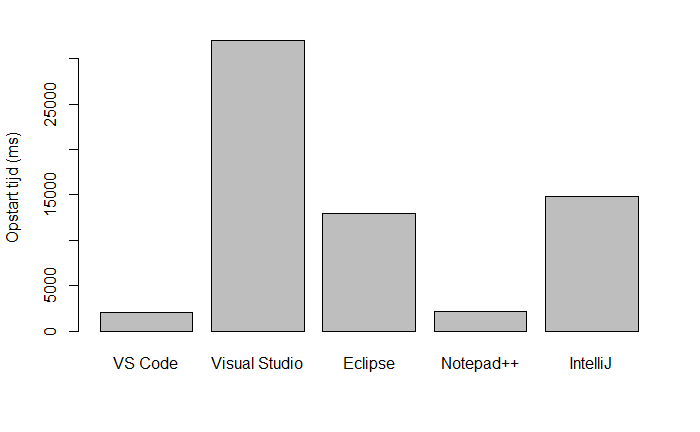
\includegraphics[width=1\linewidth]{StartupTime.png}
        \vspace*{-1.4cm}
        \caption{Gemiddelde opstarttijd}
        \label{fig:startupTime}
    \end{minipage}%
    \begin{minipage}{0.6\linewidth}
        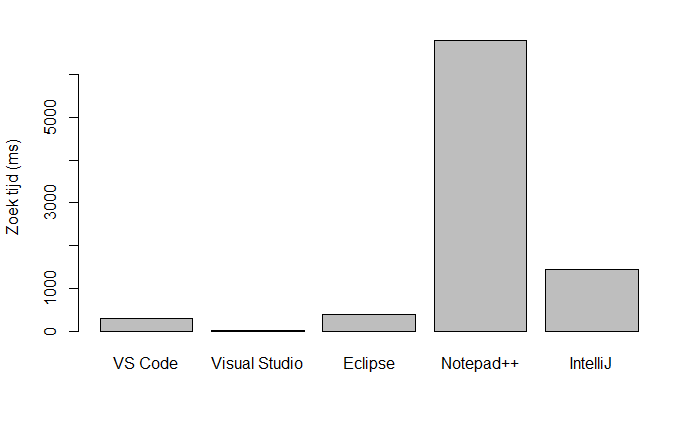
\includegraphics[width=1\linewidth]{SearchTime.png}
        \vspace*{-1.4cm}
        \caption{Gemiddelde zoektijd}
        \label{fig:searchTime}
    \end{minipage}
\end{figure}

\begin{figure}[h]
    \centering
    \addtolength{\leftskip} {-2cm}
    \addtolength{\rightskip}{-2cm}
    \begin{minipage}{0.6\linewidth}
        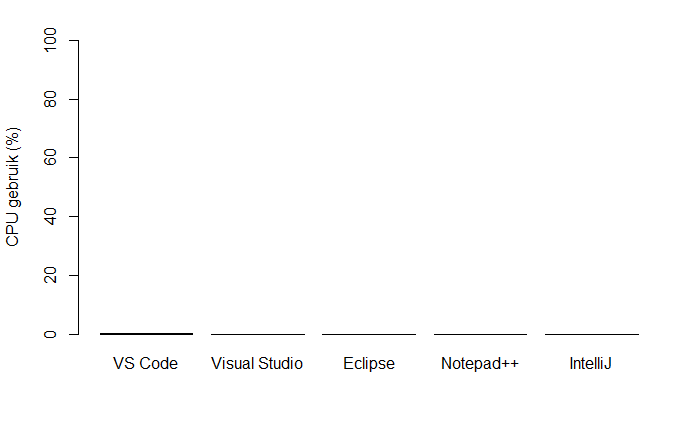
\includegraphics[width=1\linewidth]{CPUUsage.png}
        \vspace*{-1.4cm}
        \caption{Gemiddeld CPU gebruik}
        \label{fig:CPUUsage}
    \end{minipage}%
    \begin{minipage}{0.6\linewidth}
        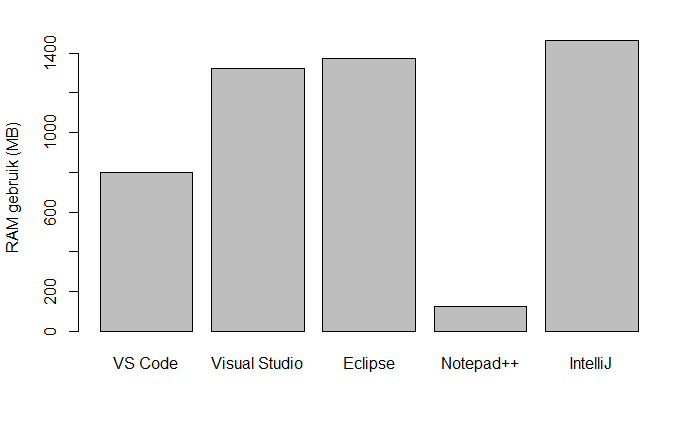
\includegraphics[width=1\linewidth]{RAMUsage.png}
        \vspace*{-1.4cm}
        \caption{Gemiddelde RAM gebruik}
        \label{fig:RAMUsage}
    \end{minipage}
\end{figure}

\begin{figure}[h!]
    \centering
    \begin{minipage}{0.6\linewidth}
        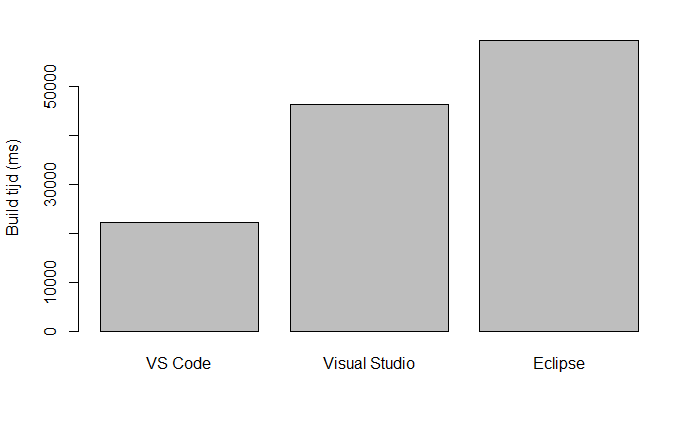
\includegraphics[width=1\linewidth]{BuildTime.png}
        \vspace*{-1.4cm}
        \caption{Gemiddelde build tijd}
        \label{fig:buildTime}
    \end{minipage}%
\end{figure}


%%=============================================================================
%% Bijlagen
%%=============================================================================

\appendix
\renewcommand{\chaptername}{Appendix}

%%---------- Onderzoeksvoorstel -----------------------------------------------

\chapter{Onderzoeksvoorstel}

Het onderwerp van deze bachelorproef is gebaseerd op een onderzoeksvoorstel dat vooraf werd beoordeeld door de promotor. Dat voorstel is opgenomen in deze bijlage.

% Verwijzing naar het bestand met de inhoud van het onderzoeksvoorstel
%---------- Inleiding ---------------------------------------------------------

\section{Introductie} % The \section*{} command stops section numbering
\label{sec:introductie}

De job van een programmeur is complex met verschillende verantwoordelijkheden. Dit gaat van het effectieve schrijven van nieuwe code tot het testen van deze code, het opsporen van fouten, het beheren van verschillende versies... Om deze lasten te verminderen zijn er over de jaren heen verschillende geïntegreerde ontwikkelingsomgeving (IDEs) op de markt gekomen, met het doel de productiviteit van de programmeur te verhogen. 

IDEs zijn ver gekomen sinds het idee ten eerste werd voorgesteld in de 1980 \autocite{Kline2005}. De eerste versies waren onhandig in gebruik en vereisten meerdere uren professionele training om effectief gebruikt te kunnen worden. Deze programma’s hadden wel het potentieel om programmeurs productiever te laten worden, maar door de grote leercurve verkozen vele de gewone tekst-editor. De kost van de eerste software was ook een grote barrière, deze kon makkelijk oplopen tot \$20,000 per ontwikkelaar. Hedendaags gebruikt bijna iedere programmeur een IDE en deze zijn vaak gratis en open source. 

In dit onderzoek wordt getracht te achterhalen hoe het met de markt van gratis IDEs gesteld is, op vlakken van hardware vereisten, leercurve, functionaliteit, configuratie en extensies. Daarnaast word onderzocht in welke use cases beginnende en ervaren programmeurs de betalende software beter ervaren.

%---------- Stand van zaken ---------------------------------------------------

\section{State-of-the-art}
\label{sec:state-of-the-art}

De hoofdfunctie van de geïntegreerde ontwikkelingsomgeving is de broncode-editor, deze is meestal voorzien van syntax markering, auto aanvulling en code controle. Daarnaast heeft de moderne IDE een ingebouwde debugger en versie controlesysteem. Momenteel is de populairste IDE Visual Studio Code \autocite{StackOverflow2021}, deze gratis software is vooral populair door zijn kleine leercurve en ecosysteem van extensies. Een andere populaire gratis IDE is Eclipse, deze is gespecialiseerd in Java, maar heeft vele extensie voor andere programmeertalen. Visual Studio 2019 is een betalende IDE, met een gratis versie, en heeft ingebouwde ondersteuning voor C, C++, C\#, F\#, TypeScript, XML en HTML. Een andere populaire optie zijn de IDEs van JetBrains, dit bedrijf biedt meerder betalende IDEs aan met bijvoorbeeld IntelliJ voor Java-applicaties en Rider voor C++ applicaties.

In het verleden zijn er al gebruiksanalyses van Eclipse en Visual Studio geweest \autocite{Murphy2006, Amann2016}. Hier werd er passief opgenomen welke functionaliteiten van de IDE de programmeurs meest gebruikten, maar er is nog geen onderzoek gebeurd naar wat programmeurs zelf waarderen in IDEs. 

Er is geen bestaand onderzoek over de hardware requirements van IDEs en hoe de verschillende programma’s hier zich van elkaar onderscheiden. Het is wel algemeen aanvaard dat voor sommige projecten de hardware requirements zeer hoog worden. Over dit onderwerp is er al onderzoek gebeurd voor het migreren van desktop gebaseerde IDEs naar de cloud \autocite{Devadiga2021}.

% Voor literatuurverwijzingen zijn er twee belangrijke commando's:
% \autocite{KEY} => (Auteur, jaartal) Gebruik dit als de naam van de auteur geen onderdeel is van de zin.
% \textcite{KEY} => Auteur (jaartal)  Gebruik dit als de auteursnaam wel een functie heeft in de zin (bv. ``Uit onderzoek door Doll & Hill (1954) bleek  ...'')

%---------- Methodologie ------------------------------------------------------
\section{Methodologie}
\label{sec:methodologie}

Dit onderzoek zal bestaan uit zowel een vragenlijst als technische experimenten. De vragenlijst die zal opgesteld worden zal ingevuld worden door zowel beginnende als ervaren programmeurs. Deze vragenlijst zal nagaan welke eigenschappen elke programmeur belangrijk acht, en welke functionaliteiten men dagelijks gebruikt. Daarnaast zal er ook gevraagd worden met welke IDEs men ervaring heeft en welke men verkiest. Ten laatste zal er nagegaan worden welke problemen men ondervindt in het dagelijkse gebruik van IDEs en wat men mist van functionaliteit.

De technische experimenten zullen bestaan in het meten van opstart en compileer -tijden in zowel run als debug configuratie, en het systeemverbruik bij normaal gebruik en op de achtergrond. Hiervoor zullen 3 projecten gebruikt worden: een leeg project met geen code, een project met een applicatie van gemiddelde grote, en een zware applicatie met meerdere dependencies. De IDEs die opgenomen zullen worden in het onderzoek zijn: Visual Studio Code, Eclipse, Visual Studio 2019 Community, Visual Studio 2019 Enterprise met en zonder dotUltimate extensies, Rider en IntelliJ.



%---------- Verwachte resultaten ----------------------------------------------
\section{Verwachte resultaten}
\label{sec:verwachte_resultaten}

De auteur verwacht dat beginnende gebruikers vooral de auto aanvulling en code controle belangrijk zullen vinden. De auteur verwacht ook dat de ervaren gebruikers dezelfde functionaliteiten belangrijk zullen vinden met daarnaast de geavanceerdere features die voornamelijk helpen bij het beheren van een grote code base die vooral voorkomen in de gespecialiseerde betalende IDEs.

Voor de technische experimenten verwacht de auteur dat Visual Studio Code het beste zal scoren op opstart en compileer -tijden maar dat het resource verbruik bij normaal gebruik en op de achtergrond het grootste zal zijn. De andere IDEs zullen meer tijd in beslag nemen om op te starten maar de compileer tijden zullen gelijkaardig zijn.



%---------- Verwachte conclusies ----------------------------------------------
\section{Verwachte conclusies}
\label{sec:verwachte_conclusies}

De verwachte resultaten leiden er toe dat Visual Studio Code de aanbevolen IDE is voor de gemiddelde programmeur, zoals de huidige markt weerspiegeld. Voor sommige gebruikers kan het wel voordelig zijn om gespecialiseerde IDEs aan te schaffen, maar enkel als hier een specifieke nood toe is.



%%---------- Andere bijlagen --------------------------------------------------
% TODO: Voeg hier eventuele andere bijlagen toe
%\input{...}
%%=============================================================================
%% Bijlange
%%=============================================================================


\chapter{\IfLanguageName{dutch}{Bijlagen}{Introduction}}
\section{Task.Json}
\label{b:taskJson}

\begin{verbatim}
{
    "version": "2.0.0",
    {
        "label": "build",
        "command": "dotnet",
        "type": "process",
        "args": [
            "build",
            "${workspaceFolder}/src/Cake.sln"
        ],
        "problemMatcher": "$msCompile"
    }
    ]
}    
\end{verbatim}

%%---------- Referentielijst --------------------------------------------------

\printbibliography[heading=bibintoc]

\end{document}
